\section{Resultate}
\label{sec:Resultate}

\subsection{Pooltemperatur}
\label{subsec:Pooltemperatur}
In der Abbildung \ref{fig:pool-temp} ist die Wassertemperatur in Abhängigkeit der Zeit dargestellt.
 
\begin{figure}[H]
	\centering
	\includegraphics[width=\linewidth]{pool-temp}
	\caption{Pooltemperatur in Abhängigkeit der Zeit}
	\label{fig:pool-temp}
\end{figure}

Aus dem Bild lässt sich herauslesen, dass der Pool die Temperatur von 30\,°C nach ungefähr 13 Tagen und 7 Stunden erreicht. Danach bewegt sich die Temperatur im vorgegebenen Bereich von 29.5\,°C bis 30.5\,°C. Dies entspricht den erwarteten Werten. Bei genauerer Betrachtung lässt sich allerdings eine minimale Temperatur von 29.4\,°C messen. Dies liegt daran, dass die Heizung erst einschaltet, wenn die Pooltemperatur 29.5\,°C unterschreitet und das System sehr träge ist.

\subsection{Regelung}
\label{subsec:Regelung}
Abbildung \ref{fig:heizung} zeigt auf, wann die Heizung eingeschaltet ist und wann nicht.

\begin{figure}[H]
	\centering
	\includegraphics[width=\linewidth]{heizung}
	\caption{Verhalten der geregelten Heizung}
	\label{fig:heizung}
\end{figure}

Vergleicht man den Verlauf dieser Kurve mit der Wassertemperatur (Abb. \ref{fig:pool-temp}), so kann man sehen, dass die Heizung eingeschaltet wird, sobald die Temperatur unter 29.5\,°C sinkt. Weiter wird die Heizung ausgeschaltet, wenn die Temperatur über 30.5\,°C steigt. Mit diesem Verlauf wäre man in der Lage, die Heizkosten eines Pools ungefähr zu bestimmen.

\subsection{Umwelteinflüsse}
\label{subsec:Umwelteinfluesse}
Abbildung \ref{fig:umgebung-hitze} zeigt den Wärmefluss der verschiedenen Umwelteinflüsse in Abhängigkeit der Zeit. Dabei bedeutet ein positiver Wärmefluss, dass dem Pool Energie zugeführt wird. Ein negativer Wärmefluss bedeutet hingegen, dass dem Pool Energie entzogen wird.

\begin{figure}[H]
	\centering
	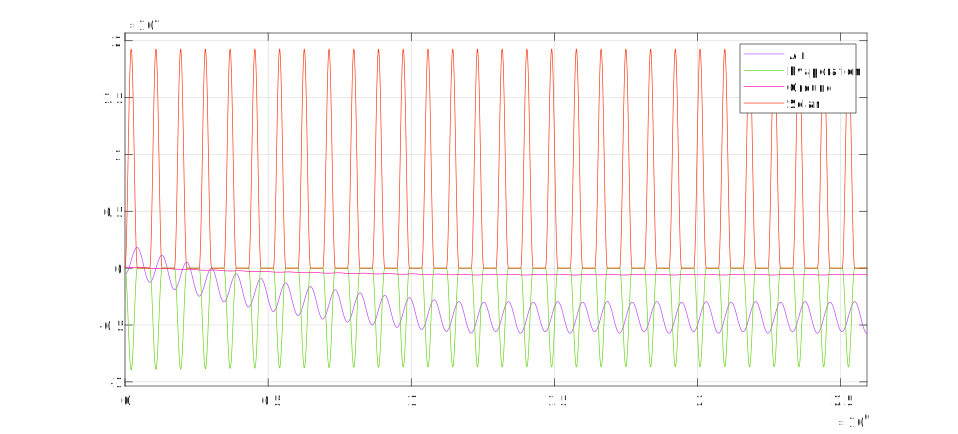
\includegraphics[width=\linewidth]{umgebung-hitze}
	\caption{Wärmefluss der verschiedenen Umwelteinflüsse in Abhängigkeit der Zeit (s)}
	\label{fig:umgebung-hitze}
\end{figure}

Auffällig ist, dass die Luft zu Beginn der Aufheizphase noch Energie zuführt, danach aber nur noch Energie entzieht. Dies liegt an der tiefen Wassertemperatur am Anfang der Simulation (nur 10\,°C). Nach drei Tagen ist die Wassertemperatur vom Pool höher als die Lufttemperatur und es wird nur noch Energie entzogen.

Durch das Mitteln der Kurven kann man bestimmen, welche durchschnittliche Leistung durch die entsprechenden Umwelteinflüsse verloren geht:

\begin{table}[H]
	\centering
	\renewcommand{\arraystretch}{1.2}
	\begin{tabular}{L{6.5cm}cr}
		Konvektion (Wasser zu Luft)		& -			& 4340\,W				\\
		Wasserverdunstung 				& -			& 2232\,W				\\
		Wärmeleitung (Wände und Boden)	& -			& 575\,W				\\
		Sonneneinstrahlung				& +			& 4817\,W				\\ \hline
		\textbf{Total}    				& \textbf{-} 	& \textbf{2330\,W}
	\end{tabular}                                                           
\end{table}

\subsection{Zeitabschätzung}
\label{subsec:Zeitabschaetzung}
Zuerst wurde eine grobe Abschätzung der Aufheizzeit vorgenommen, welche als Anhaltspunkt dient (siehe Angang \ref{app:Zeitabschaetzung}). In dieser Zeitabschätzung wurden die verschiedenen Umwelteinflüsse komplett vernachlässigt. Es wurde eine Aufheizzeit von 13 Tagen und 8 Stunden berechnet, welche sehr gut mit der Simulation übereinstimmt. Dies bedeutet, dass sich die Umwelteinflüsse während der Aufheizphase gegenseitig fast aufheben.
